% Author: Izaak Neutelings (February 2020)
\documentclass[border=3pt,tikz]{standalone}
\usepackage{physics}
\usepackage{xcolor}
\usetikzlibrary{decorations.markings}
\usetikzlibrary{hobby}
\tikzset{>=latex} % for LaTeX arrow head

\colorlet{Ecol}{orange!90!black}
\colorlet{Bcol}{violet!90}
\colorlet{Icol}{blue!70!black}
\colorlet{gausscol}{green!40!black}
\colorlet{gausscol2}{green!45!blue}
\tikzstyle{current}=[->,Icol,thick]
\colorlet{pluscol}{red!60!black}
\colorlet{minuscol}{blue!60!black}
\tikzstyle{anode}=[top color=red!20,bottom color=red!50,shading angle=20]
\tikzstyle{cathode}=[top color=blue!20,bottom color=blue!40,shading angle=20]
\tikzstyle{gauss surf}=[gausscol,top color=green!2,bottom color=green!80!black!70,shading angle=5,fill opacity=0.4]
\tikzstyle{metal}=[top color=black!15,bottom color=black!25,middle color=black!20,shading angle=10]
\tikzstyle{mydashes}=[dash pattern=on 1 off 1]
\tikzset{
  EFieldLine/.style={thick,Ecol,line cap=round,decoration={markings,
                     mark=at position #1 with {\arrow{latex}}},
                     postaction={decorate}},
  BFieldLine/.style={thick,Bcol,postaction={decorate},decoration={markings,
                     mark=at position #1 with {\arrow{latex}},
                     mark=at position #1+0.5 with {\arrow{latex}}}},
  EFieldLine/.default=0.5,
  BFieldLine/.default=0.4}
\usetikzlibrary{3d}

\begin{document}


% CAPACITOR 3D - displacement current derivation
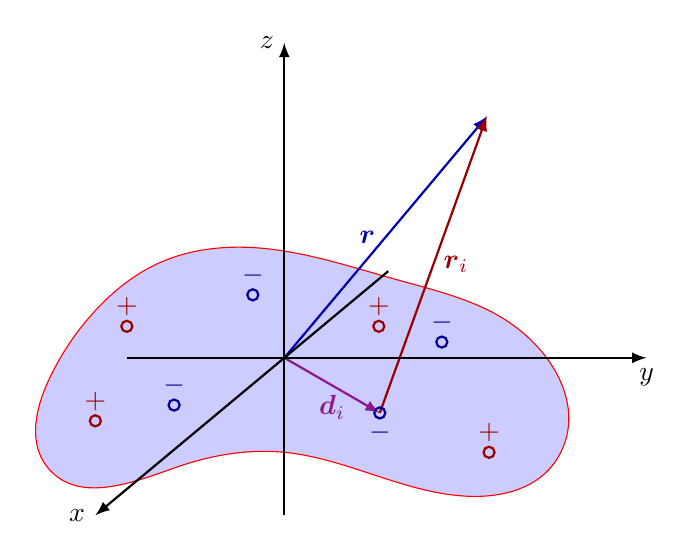
\begin{tikzpicture}[scale=2]
    \def\R{2}
    \coordinate (P) at (50:\R);
    \coordinate (Q) at (-30:0.7);
     \draw[red, fill=blue!20, use Hobby shortcut,closed=true]
        (-1.5,-.15) .. (-1.2,.3) .. (-0.8,.6) .. 
        (-.2,0.7) .. (0.7,.5) .. (1.3,.3)  .. (1.72,-0.66) ..
        (1.2,-0.88) .. (0,-.6) .. (-.7,-.7) .. (-1.5,-.7);
    \draw [thick, Icol, ->] (0,0) --node [left] {$\boldsymbol{r}$} (P);
    \draw [thick, Bcol, ->] (0,0) --node [below] {$\boldsymbol{d}_i$} (Q);
    \draw [thick, pluscol, ->] (Q) --node [right] {$\boldsymbol{r}_i$} (P);
    \draw[thick, -latex] (-1, 0) -- (2.3, 0) node [below] {$y$};
    \draw[thick, -latex] (0, -1) -- (0, 2) node [left] {$z$};
    \draw[thick, -latex]  (0.66, 0.55) -- (-1.2, -1) node [left] {$x$};

    \draw[pluscol, thick] (-1, 0.2) circle (1pt) node [above] {$+$};
    \draw[minuscol, thick] (Q) circle (1pt) node [below] {$-$};
    \draw[pluscol, thick] (-1.2, -0.4) circle (1pt) node [above] {$+$};
    \draw[minuscol, thick] (-0.7, -0.3) circle (1pt) node [above] {$-$};
    \draw[pluscol, thick] (0.6, 0.2) circle (1pt) node [above] {$+$};
    \draw[minuscol, thick] (-0.2, 0.4) circle (1pt) node [above] {$-$};
    \draw[minuscol, thick] (1, 0.1) circle (1pt) node [above] {$-$};
    \draw[pluscol, thick] (1.3, -0.6) circle (1pt) node [above] {$+$};

   
    
\end{tikzpicture}
  
\end{document}